\scanpage{21}

\unsure{l'ens|lieu} des $p$ de $\operatorname{Spec}A$ où $B$ l'est est-il
ouvert? ]. Il \unsure{faudra|faut} supposer que $A$ et $B$
sont des ``bons anneaux''.

En particulier, l'\unsure{énoncé précédent} est-il
\deleted{$A,B$ \unsure{sont locaux}, $A\unsure{\longrightarrow|\text{---}}B$}
stable par localisation ?
\margin{Cf IV \unsure{2.10.1|2.40.1}}
\figure{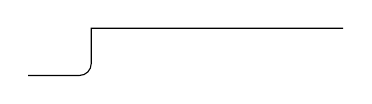
\begin{tikzpicture}\draw (0,0)--(.65,0) to[out=0,in=-90] (.8,.15)--(.8,.6)--(4,.6);\end{tikzpicture}}

\margin{On est ramené au cas où $A$ est \uline{intègre}; à \unsure{prouver}
(a) si $x\in U$, \unsure{pour} \unsure{tte} \unsure{générisation}
\unsure{au dessus de} $\unsure{x}$, $\unsure{x\longrightarrow y}$, $y\in U$.
(b) \deleted{Si $x\in U$, \unsure{son} \unsure{adhérence} \unsure{est} \unsure{contenue dans}}
\deleted{Si $x\in U$} $\unsure{U}$ est \unsure{dense en} $\unsure{\overline{\{y\}}}$,
\unsure{alors} \unsure{il} contient un \unsure{voisinage} de $\unsure{x}$
\unsure{dans} $\unsure{\overline{\{x\}}}$ \unsure{qui est dans} $U$.}
\margin{\figure{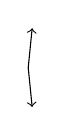
\begin{tikzpicture}\draw[<->] (0,1)--(-.05,.5)--(0,0);\end{tikzpicture}}}

Le cas d'extensions résiduelles finies.
cf critère jacobien de Nagata et
th. de Nagata pour une algèbre locale noeth
complète sur un \uline{corps}.

OK. en caractéristique 0 pour les \uline{bons
anneaux}, grâce à la \uline{résolution des
singularités}.

\margin{Pour (b), dans le cas d'un bon anneau,
on est ramené au cas où $B$ est \uline{régulier}. \unsure{Alors},
\unsure{a)} \unsure{reste une} \unsure{hypothèse de}
la résolution des singularités, et
\unsure{pour a)} \unsure{se résout par} \uline{l'affirmative}.
\unsure{En réalité}, il se résout par l'affirmative
pour les bons anneaux, \uline{en \unsure{caractéristique} \unsure{entière|quelconque}},
\uline{\unsure{pourvu qu'on sache}}
\unsure{que le} \unsure{lieu où} un $f$ sur $X$
est \unsure{géométriquement} \unsure{régulier}
est \uline{ouvert} (au \unsure{moins} \unsure{au-dessus de} $k$).}

4) $A\unsure{\text{---}|\longrightarrow}B$ hom d'anneaux
noeth. Lieu des $\unsure{q|p}$ de
$\operatorname{Spec}B$ en lesquels $B$ est plat
sur $A$ est-il ouvert?
[Ceci revient à vérifier
que pour $\forall p\in\operatorname{Spec}A$,
et $\forall q$ au dessus de $p$,
maximal parmi \unsure{ceux-là|ceux-ci},
posant $A'=A/p$, $B'=B/q$
\inserted{$A'\subset B'$ intègres}
[\unsure{donc} $B'\otimes_{A'}K'$ \unsure{est un corps}]
$\exists$ un ouvert non vide de $\operatorname{Spec}B'$
en \unsure{lesquels|lequel} $B'$ est plat sur $A'$.
\figure{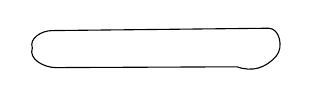
\begin{tikzpicture}\draw (0,.2) to[out=110,in=180] (.25,.42)--(3,.45) to[out=0,in=50] (3.1,.1) to[out=230,in=-20] (2.6,-.04)--(.3,-.05) to[out=180,in=-110] (0,.2);\end{tikzpicture}}

\begin{center}
M. DUFOUR\\
VARITYPISTE\\
131, RUE LECOURBE\\
PARIS XV$^{\mathrm e}$\\
\figure{\begin{tikzpicture}\fill (0,0) rectangle (.12,.12);\end{tikzpicture}}\\
C. C. P. Paris \unsure{14.143.34|14.143-34}\\
R. M. 140.029
\end{center}

\mspage{20}
